\documentclass[12pt]{article}
\usepackage{xcolor}
\usepackage{amsmath, mathtools}
\usepackage{amsfonts}
\usepackage{amssymb}
\usepackage{graphicx}
\usepackage{colortbl}
\usepackage{xr}
\usepackage{hyperref}
\usepackage{longtable}
\usepackage{xfrac}
\usepackage{tabularx}
\usepackage{float}
\usepackage{siunitx}
\usepackage{booktabs}
\usepackage{caption}
\usepackage{pdflscape}
\usepackage{afterpage}
\usepackage{comment}
\usepackage{hyperref}

\usepackage[round]{natbib}

%\usepackage{refcheck}

\hypersetup{
    bookmarks=true,         % show bookmarks bar?
      colorlinks=true,       % false: boxed links; true: colored links
    linkcolor=red,          % color of internal links (change box color with linkbordercolor)
    citecolor=green,        % color of links to bibliography
    filecolor=magenta,      % color of file links
    urlcolor=cyan           % color of external links
}

%% Comments

\usepackage{color}

\newif\ifcomments\commentstrue

\ifcomments
\newcommand{\authornote}[3]{\textcolor{#1}{[#3 ---#2]}}
\newcommand{\todo}[1]{\textcolor{red}{[TODO: #1]}}
\else
\newcommand{\authornote}[3]{}
\newcommand{\todo}[1]{}
\fi

\newcommand{\wss}[1]{\authornote{blue}{SS}{#1}}
\newcommand{\an}[1]{\authornote{magenta}{Malavika}{#1}}


% For easy change of table widths
\newcommand{\colZwidth}{1.0\textwidth}
\newcommand{\colAwidth}{0.13\textwidth}
\newcommand{\colBwidth}{0.82\textwidth}
\newcommand{\colCwidth}{0.1\textwidth}
\newcommand{\colDwidth}{0.05\textwidth}
\newcommand{\colEwidth}{0.8\textwidth}
\newcommand{\colFwidth}{0.17\textwidth}
\newcommand{\colGwidth}{0.5\textwidth}
\newcommand{\colHwidth}{0.28\textwidth}

% Used so that cross-references have a meaningful prefix
\newcounter{defnum} %Definition Number
\newcommand{\dthedefnum}{GD\thedefnum}
\newcommand{\dref}[1]{GD\ref{#1}}
\newcounter{datadefnum} %Datadefinition Number
\newcommand{\ddthedatadefnum}{DD\thedatadefnum}
\newcommand{\ddref}[1]{DD\ref{#1}}
\newcounter{theorynum} %Theory Number
\newcommand{\tthetheorynum}{T\thetheorynum}
\newcommand{\tref}[1]{T\ref{#1}}
\newcounter{tablenum} %Table Number
\newcommand{\tbthetablenum}{T\thetablenum}
\newcommand{\tbref}[1]{TB\ref{#1}}
\newcounter{assumpnum} %Assumption Number
\newcommand{\atheassumpnum}{P\theassumpnum}
\newcommand{\aref}[1]{A\ref{#1}}
\newcounter{goalnum} %Goal Number
\newcommand{\gthegoalnum}{P\thegoalnum}
\newcommand{\gsref}[1]{GS\ref{#1}}
\newcounter{instnum} %Instance Number
\newcommand{\itheinstnum}{IM\theinstnum}
\newcommand{\iref}[1]{IM\ref{#1}}
\newcounter{reqnum} %Requirement Number
\newcommand{\rthereqnum}{P\thereqnum}
\newcommand{\rref}[1]{R\ref{#1}}
\newcounter{lcnum} %Likely change number
\newcommand{\lthelcnum}{LC\thelcnum}
\newcommand{\lcref}[1]{LC\ref{#1}}

\newcommand{\famname}{CFS} % PUT YOUR PROGRAM NAME HERE

\usepackage{fullpage}

\begin{document}

\title{Curve Fitting Software} 
\author{Malavika Srinivasan}
\date{\today}

\maketitle

~\newpage

\pagenumbering{roman}

\section{Revision History}

\begin{tabularx}{\textwidth}{p{3cm}p{2cm}X}
\toprule {\bf Date} & {\bf Version} & {\bf Notes}\\
\midrule
Sep 28, 2018 & 1.0 & First draft by Malavika\\
Date 2 & 1.1 & Notes\\
\bottomrule
\end{tabularx}

~\newpage
	
\section{Reference Material}

This section records information for ease of reference. The information includes the units, symbols and abbreviations used in this document.

\subsection{Table of Units}
This library is designed to work for any set of data, irrespective of their units. So, table of units is not applicable. 
\begin{comment}


Throughout this document SI (Syst\`{e}me International d'Unit\'{e}s) is employed
as the unit system.  In addition to the basic units, several derived units are
used as described below.  For each unit, the symbol is given followed by a
description of the unit and the SI name.
~\newline

\renewcommand{\arraystretch}{1.2}
%\begin{table}[ht]
  \noindent \begin{tabular}{l l l} 
    \toprule		
    \textbf{symbol} & \textbf{unit} & \textbf{SI}\\
    \midrule 
    \si{\metre} & length & metre\\
    \si{\kilogram} & mass	& kilogram\\
    \si{\second} & time & second\\
    \si{\celsius} & temperature & centigrade\\
    \si{\joule} & energy & Joule\\
    \si{\watt} & power & Watt (W = \si{\joule\per\second})\\
    \bottomrule
  \end{tabular}
  %	\caption{Provide a caption}
%\end{table}

\wss{Only include the units that your CA actually uses.  If there are no units
  for your problem, like for a general purpose library, you should still include
the heading, with the content ``not applicable'' (or similar).}
\end{comment}
\subsection{Table of Symbols}

The table that follows summarizes the symbols used in this document along with
their units. The symbols are listed in alphabetical order.
\ms{I am just noting down symbols, they are not yet in alphabetical order}
\renewcommand{\arraystretch}{1.2}
%\noindent \begin{tabularx}{1.0\textwidth}{l l X}
\noindent \begin{longtable*}{l l p{12cm}} \toprule
\textbf{symbol} & \textbf{unit} & \textbf{description}\\
\midrule 

$A_\text{in}$ & \si[per-mode=symbol] {\square\metre} & \\
$\Phi$ & & \\
$\sum_{min}^{max}$& & \\
 
\bottomrule
\end{longtable*}
\ms{ISSUE 1: For libraries, we have only mathematical symbols which do not have units. Should we remove units or just say not applicable.}
\wss{Use your problems actual symbols.  The si package is a good idea to use for
  units.}

\subsection{Abbreviations and Acronyms}

\renewcommand{\arraystretch}{1.2}
\begin{tabular}{l l} 
  \toprule		
  \textbf{symbol} & \textbf{description}\\
  \midrule 
  A & Assumption\\
  DD & Data Definition\\
  GD & General Definition\\
  GS & Goal Statement\\
  IM & Instance Model\\
  LC & Likely Change\\
  PS & Physical System Description\\
  R & Requirement\\
  %SRS & Software Requirements Specification\\
  CA & Commonality Analysis\\
  \famname & Curve Fitting Software\\
  T & Theoretical Model\\
  \bottomrule
\end{tabular}\\

\wss{Add any other abbreviations or acronyms that you add}

\newpage

\tableofcontents

~\newpage

\pagenumbering{arabic}

\section{Introduction}

Scientific Computation (SC) is the collection of tools, techniques, and theories that are required to solve problems in the field of science and engineering using computer-based mathematical models. The source data for scientific computation problems are often large sets of data from experiments conducted in a laboratory setup. This large set of data (such as time and temperature) is usually complex to analyze and require segmenting and curve-fitting.

Curve fitting is the process of constructing a curve, or mathematical function, that has the best fit to a series of data points possibly subject to constraints~\cite{CurvefitWiki}.
\begin{figure}[h!]
	\begin{center}
		%rotatebox{-90}
		{
			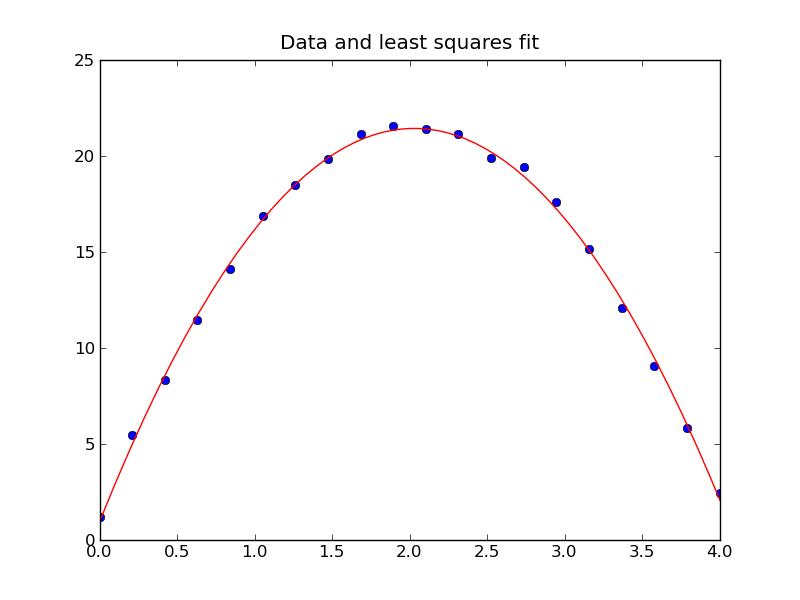
\includegraphics[width=0.5\textwidth]{lstsq11.png}
		}
		\caption{\label{Fig_CurveFitEg} Typical example of a curve fitting process}
	\end{center}
\end{figure}

A fit for the data can be obtained by different methods like interpolation, data smoothing and regression.

\subsection{Interpolation}
Interpolation is a process of fitting a function to given data so that the function has some values as the given data.

\subsection{Smoothing}
Smoothing is a process of creating an approximating function that attempts to capture important patterns in the data, while leaving out noise or other rapid phenomena.

\subsection{Regression}
Regression analysis is the process of finding the best fit parameters for a regression model for a given set of data points and thus obtain a curve through a set of data points. \\ 






\subsection{Purpose of Document}


\subsection{Scope of the Family} 

\subsection{Characteristics of Intended Reader} 

\subsection{Organization of Document}

\section{General System Description}

This section identifies the interfaces between the system and its environment,
describes the potential user characteristics and lists the potential system
constraints.

\subsection{Potential System Contexts}

\wss{Your system context will likely include an explicit list of user and system
  responsibilities}

\begin{itemize}
\item User Responsibilities:
\begin{itemize}
\item 
\end{itemize}
\item \famname{} Responsibilities:
\begin{itemize}
\item Detect data type mismatch, such as a string of characters instead of a
  floating point number
\item 
\end{itemize}
\end{itemize}

\subsection{Potential User Characteristics} \label{SecUserCharacteristics}

The end user of \famname{} should have an understanding of undergraduate Level
1 Calculus and Physics.

\subsection{Potential System Constraints}

\wss{You may not have any system constraints}

\section{Commonalities}

\subsection{Background Overview} \label{Sec_Background}

\subsection{Terminology and  Definitions}

This subsection provides a list of terms that are used in the subsequent
sections and their meaning, with the purpose of reducing ambiguity and making it
easier to correctly understand the requirements:

\begin{itemize}

\item 

\end{itemize}

\subsection{Data Definitions} \label{sec_datadef}

This section collects and defines all the data needed to build the instance
models. The dimension of each quantity is also given.  \wss{Modify the examples
  below for your problem, and add additional definitions as appropriate.}

~\newline

\noindent
\begin{minipage}{\textwidth}
\renewcommand*{\arraystretch}{1.5}
\begin{tabular}{| p{\colAwidth} | p{\colBwidth}|}
\hline
\rowcolor[gray]{0.9}
Number& DD\refstepcounter{datadefnum}\thedatadefnum \label{FluxCoil}\\
\hline
Label& \bf Heat flux out of coil\\
\hline
Symbol &$q_C$\\
\hline
% Units& $Mt^{-3}$\\
% \hline
  SI Units & \si{\watt\per\square\metre}\\
  \hline
  Equation&$q_C(t) = h_C (T_C - T_W(t))$, over area $A_C$\\
  \hline
  Description & 
                $T_C$ is the temperature of the coil (\si{\celsius}).  $T_W$ is the temperature of the water (\si{\celsius}).  
                The heat flux out of the coil, $q_C$ (\si{\watt\per\square\metre}), is found by
                assuming that Newton's Law 
                of Cooling applies (\aref{A_Newt_coil}).  This law (\dref{NL}) is used on the surface of
                the coil, which has area $A_C$ (\si{\square\metre}) and heat 
                transfer coefficient $h_C$
                (\si{\watt\per\square\metre\per\celsius}).  This equation
                assumes that the temperature of the coil is constant over time (\aref{A_tcoil}) and that it does not vary along the length
                of the coil (\aref{A_tlcoil}).
  \\
  \hline
  Sources& Citation here\\
  \hline
  Ref.\ By & \iref{ewat}\\
  \hline
\end{tabular}
\end{minipage}\\

\subsection{Goal Statements}

\noindent Given the \wss{inputs}, the goal statements are:

\begin{itemize}

\item[GS\refstepcounter{goalnum}\thegoalnum \label{G_meaningfulLabel}:] \wss{One
    sentence description of the goal.  There may be more than one.  Each Goal
    should have a meaningful label.}

\end{itemize}

\subsection{Theoretical Models} \label{sec_theoretical}

This section focuses on the general equations and laws that \famname{} is based
on.  \wss{Modify the examples below for your problem, and add additional models
  as appropriate.}

~\newline

\noindent
\begin{minipage}{\textwidth}
\renewcommand*{\arraystretch}{1.5}
\begin{tabular}{| p{\colAwidth} | p{\colBwidth}|}
  \hline
  \rowcolor[gray]{0.9}
  Number& T\refstepcounter{theorynum}\thetheorynum \label{T_COE}\\
  \hline
  Label&\bf Conservation of thermal energy\\
  \hline
  Equation&  $-{\bf \nabla \cdot q} + g$ = $\rho C \frac{\partial T}{\partial t}$\\
  \hline
  Description & 
                The above equation gives the conservation of energy for transient heat transfer in a material
                of specific heat capacity $C$ (\si{\joule\per\kilogram\per\celsius}) and density $\rho$ 
                (\si{\kilogram\per\cubic\metre}), where $\bf q$ is the thermal flux vector (\si{\watt\per\square\metre}),
                $g$ is the volumetric heat generation
                (\si{\watt\per\cubic\metre}), $T$ is the temperature
                (\si{\celsius}),  $t$ is time (\si{\second}), and $\nabla$ is
                the gradient operator.  For this equation to apply, other forms
                of energy, such as mechanical energy, are assumed to be negligible in the
                system (\aref{A_OnlyThermalEnergy}).  In general, the material properties ($\rho$ and $C$) depend on temperature.\\
  \hline
  Source &
           \url{http://www.efunda.com/formulae/heat_transfer/conduction/overview_cond.cfm}\\
  % The above web link should be replaced with a proper citation to a publication
  \hline
  Ref.\ By & \dref{ROCT}\\
  \hline
\end{tabular}
\end{minipage}\\

~\newline

\section{Variabilities}

\subsection{Assumptions}

\begin{itemize}

\item[A\refstepcounter{assumpnum}\theassumpnum \label{A_meaningfulLabel}:]
  \wss{Short description of each assumption.  Each assumption
    should have a meaningful label.  Use cross-references to identify the
    appropriate traceability to T, GD, DD etc., using commands like dref, ddref etc.}

\end{itemize}

\subsection{Calculation} \label{sec_Calculation}

\subsection{Output} \label{sec_Output}    

\section{Requirements}

This section provides the functional requirements, the business tasks that the
software is expected to complete, and the nonfunctional requirements, the
qualities that the software is expected to exhibit.

\subsection{Functional Requirements}

\noindent \begin{itemize}

\item[R\refstepcounter{reqnum}\thereqnum \label{R_Inputs}:] \wss{Requirements
    for the inputs that are supplied by the user.  This information has to be
    explicit.}

\item[R\refstepcounter{reqnum}\thereqnum \label{R_OutputInputs}:] \wss{It isn't
    always required, but often echoing the inputs as part of the output is a
    good idea.}

\item[R\refstepcounter{reqnum}\thereqnum \label{R_Calculate}:] \wss{Calculation
    related requirements.}

\item[R\refstepcounter{reqnum}\thereqnum \label{R_VerifyOutput}:]
  \wss{Verification related requirements.}

\item[R\refstepcounter{reqnum}\thereqnum \label{R_Output}:] \wss{Output related
    requirements.}

\end{itemize}

\subsection{Nonfunctional Requirements}

\wss{List your nonfunctional requirements.  You may consider using a fit
  criterion to make them verifiable.}

\section{Likely Changes}    

\noindent \begin{itemize}

\item[LC\refstepcounter{lcnum}\thelcnum\label{LC_meaningfulLabel}:] \wss{If
    there is a ranking of variabilities, or combinations of variabilities, that
    are more likely, this information can be included here.}

\end{itemize}

\section{Traceability Matrices and Graphs}

\wss{You will have to add tables.}

\newpage

\bibliographystyle {plainnat}
\bibliography {../../ReferenceMaterial/References}

\newpage

\section{Appendix}

\wss{Your report may require an appendix.  For instance, this is a good point to
show the values of the symbolic parameters introduced in the report.}

\subsection{Symbolic Parameters}

\wss{The definition of the requirements will likely call for SYMBOLIC\_CONSTANTS.
Their values are defined in this section for easy maintenance.}



\ms{Points to be noted}\\
\ms{***********************************************************************}
\ms{Interpolation means fitting some function to given data so that the function has some values as the given data.}\\
The Simplest 1d interpolation is given by:\\
for a given data ($t_{i},y_{i}$), where $i = 1,2,3...m$,\\
f is an interpolating function such that, \\
\begin{equation*}
f(t_{i}) = y_i \text{where i} = 1,2...m
\end{equation*}

Some of the variabilities includes:\\
\begin{itemize}
	\item What form should the function have?
	\item How should the function behave between data points?
	\item Should the function inherit properties of the data such as monotonicity, convexity or periodicity?
	\item Are we interested in the values of the parameters that define the interpolating function, or simply in evaluating the function at various points for plotting or other purposes?
	\item If the function and data are plotted, should the results be visually pleasing?  
\end{itemize}

\section{Selection of function}
The selection of function for interpolation depends on the following factors:
\begin{itemize}
	\item How easy is the interpolant or the function is to work with. Working means determining the parameters of the interpolant from the data, evaluating the interpolant at a given point, differentiating or integrating the interpolant.
	\item How well the properties of the interpolant match the properties of the data to be fit(smoothness, monotonicity, convexity, periodicity etc)
\end{itemize}

Some of the familiar functions commonly used for interpolation are:
\begin{itemize}
	\item Polynomials
	\item Piecewise Polynomials
	\item Trignometric functions
	\item Exponential functions
	\item Rational functions
\end{itemize}
\ms{Questions: Ask Dr.Smith if we need to have all these five variabilities for fitting data or its enough if we have piecewise and polynomial}

To find an interpolating function for a set of data points, it is important to make sure that the interpolant exists. This comes down to the discussion of matching the number of parameters in the interpolant to number of data points to be fit.If there are too few parameters, then the interpolant does not exist. If there are too many points, then the interpolant is not unique. \\

For a gien set of data points $(t_i,y_i)$, where i $= 1,2 3...m$, an interpolant is chosen from a suitable set of basis functions $\Phi(t), \Phi_1(t), ... \Phi_n(t)$. Therefore, the interpolating function f can be expressed as a linear combination of these basis functions.

\begin{equation*}
f(t) = \sum_{j=1}^{n}x_j \Phi_j (t) 
\end{equation*}
where $x_j$ are the parameters to be found. But inorder for f to be interpolating the data points $(t_i,y_i)$, 
\begin{equation*}
f(t_i) = \sum_{j=1}^{n}x_j \Phi_j (t) = y_i
\end{equation*}
where i $= 1,2,3...m$
This can be expressed as a liner system of equations 
\begin{equation*}
Ax = y
\end{equation*}
where A is the basis matrix whose m X n entries are given by,
\begin{equation*}
a_{ij} = \Phi_j(t_i) 
\end{equation*} 
where $a_{ij}$ is the value of $j^{th}$ basis function at $i^{th}$ data point.
\textcolor{violet}{\subsection{For my understanding}
\ms{Important points to be noted here}\\
\begin{itemize}
	\item m data points $(t_i,y_i)$ where $ i = 1.... m$
	\item n basis function $\Phi_1(t) , \Phi_2(t), \Phi_3(t)... \Phi_n(t)$
	\item f is the interpolating function
	\item f is the linear combination of basis function as shown below
	\item \begin{equation*}
	f(t_i) = \sum_{j=1}^{n}x_j \Phi_j (t) = y_i
	\end{equation*}
	Where i $= 1, 2 ..m$. Here they consider m because there are m data points
	\item $x_j$ is the parameters of the fit to be found
	\item To find $x_j$, we use matrix solving method because the above form is a system of linear equations. \begin{equation*}
	Ax = y
	\end{equation*}
	
	Where A is the basis matrix whose entries are given by $a_{ij}$ 
	\item $a_{ij}$ is given by the following equation
	\begin{equation*}
	a_{ij} = \Phi_j (ti)
	\end{equation*}
\end{itemize}}




\subsection{Polynomial interpolation}

Polynomial function has different types of basis functions.
\begin{itemize}
	\item Monomial
	\item Lagrange
	\item Newton
	\item Orthogonal
	\item Interpolating continuous functions
\end{itemize}
\ms{I have worked out only monomial, lagrange and newton}
\ms{Need to ask if Orthogonal and continous function can be left out}
\subsubsection{Monomial basis}
To interpolate n data points $(t_i,y_i)$, we choose $k = n-1$ as the maximum degree of the polynomial. We define $P_{n-1}$ as the set of polynomials of degree at most n-1 and is composed on first n monomials $\Phi_j$.
\ms{Note: n data points, n basis function, max degree of polynomial = n-1}
\begin{equation*}
\Phi_j (t) = t^{j-1} 
\end{equation*}
where j $= {1,2,...n}$\\
We can construct the polynomial from this which will have the form,\\
\begin{equation*}
P_{n-1}(t) = x_1 + x_2 t + x_3 t^2 + x_4 t^3 + ... x_n t^{n-1} 
\end{equation*}
The matrix form is given by,
\ms{To understand this, see in class notes. Example problem solved} 
\begin{equation*}
Ax = \begin{bmatrix}
1 & t_{1} & t_{1} ^2 & \dots & t_{1} ^{n-1} \\
1 & t_{2} & t_{2} ^2 & \dots & t_{2} ^{n-1} \\
\vdots & \vdots & \vdots & \vdots \\
1 & t_{n} & t_{n} ^2 & \dots & t_{n} ^{n-1} \\
\end{bmatrix}
\begin{bmatrix}
x_1  \\
x_2 \\
\vdots \\
x_n \\
\end{bmatrix} = 
\begin{bmatrix}
y_1  \\
y_2 \\
\vdots \\
y_n \\
\end{bmatrix} = y
\end{equation*} 
\ms{Note: A matrix whose columns are successive powers of some independent variable t is called Vandermonde matrix}
\ms{Assumption: The vandermonde matrix should be non singular provided $t_i$ are all distint, hence the interpolant exists.}
\ms{Cost of computing interpolant is high}

\subsubsection{Lagrange Interpolation}

For a given set of data points $(t_i,y_i)$, $i = 1,2,$ \dots n, the Lagrange polynomial of degree n-1, $P_{n-1}$ is given by,
\begin{equation*}
P_{n-1} (t) = y_1 l_1 (t) + y_2 l_2(t) + \dots y_n l_n (t).
\end{equation*}

where the basis functions(also called fundamental polynomials) for the $l_j$ is given by,
\begin{equation*}
l_j (t) =  \frac{ \Pi _{k=1, k\neq j} ^n (t - t_k)} {\Pi _{k=1,k \neq j} ^ n (t_j - t_k)} = \frac{(t - t_1)}{(t_j - t_1)}...\frac{(t - t_{j-1})}{(t_j - t_{j-1})}\frac{(t - t_{j+1})}{(t_j - t_{j+1})}... \frac{(t - t_n)}{(t_j - t_n)}
\end{equation*}
where j =$ 1,2,... n$\\
The matrix form, 
\begin{equation*}
Ax = y
\end{equation*}
A is the Identity matrix I.
\ms{Expensive to evaluate and more difficult to differentiate and integrate}
\ms{n data points, n basis function, n-1 is the maximum degree of polynomials. Refer to notes for example problem.}
\subsubsection{Newton Interpolation}

For a given set of data points $(t_i,y_i)$, $i = 1,2,$ \dots n, the newton basis function for $P_{n-1}$ is given by,
\ms{n data points, n basis points}
\begin{equation*}
\pi(t) = \Pi_{k=1}^{j-1} (t - t_k) 
\end{equation*}
where j = 1,2,....n\\
When the limits make it vacuous, the product is taken to be 1\\
Also, $\pi_j (t) = 0$ for i<j.
The polynomial $P_{n-1}$ is given by,

\begin{equation*}
P_{n-1} (t) = x_1 + x_2(t-t_1) + x_3(t-t_1)(t-t_2) + ... x_n(t-t_1)(t-t_2)...(t-t_{n-1})
\end{equation*}

The matrix form of basis in $Ax = y$ is lower triangular as $\pi_j (t) = 0$ for i<j with its entries defined by $a_{ij} = \pi_j (t_i)$

\subsection{Piecewise Polynomial Interpolation}
Even though choosing an appropriate basis function and intetpolation points mitigate the difficulties associated with 

\subsubsection{Hermite Cubic interpolation}

\subsubsection{Cubic spline interpolation}

\subsubsection{B-splines}









\ms{***********************************************************************}









\end{document}